\documentclass[10pt, conference]{IEEEtran}
\usepackage{xeCJK}
\usepackage{amsmath}
\usepackage{listings}
\usepackage{amssymb}
\usepackage{float}
\usepackage{graphicx}

% 用来断词,当出现花括号中的单词时,若遇到换行需要断词的话就只能从-处断。
\hyphenation{op-tical net-works semi-conduc-tor}

\begin{document}
    \title{Report of Chapter 6 \& 7}
    \author{\IEEEauthorblockN{林奇峰, Qifeng Lin}\IEEEauthorblockA{Student ID:17214656}}
    \date{\today}
    \maketitle

    \section{Review}
        Chapter 6 and 7 mainly demonstrate reachability properties and safety properties and both of them can be seen as the dual of each other.
        
        \subsection{Reachability Properties}
        Firstly, a reachability property states that some particular situations can be reached. It can be divided into two classes: simple reachability and conditional reachability. Simple reachability states that it can reached some states and conditional one means that under some conditions, it can reached some states.
        
        In temporal logic, reachability properties can be fined as $\textbf{EF}\phi$, where $\phi$ is a propositional formula free of temporal combinators, that is {\itshape present formual}. And often our interest is the negation of reachability properties and thus, we can write it in the form of $\neg\textbf{EF}\phi$ or the equivalent form $\textbf{AG}\neg\phi$, which is read as "along any path, at any time, not $\phi$".
        
        After giving out the expression of reachability properties in temporal logic, we can use the reachability graph to compute the reachability. There mainly exists two kinds of algorithm to deal with it: "forward chaining and backward chaining".
        
        Forward chaining method constructs a set of reachable states by compute the immediate successors of each states from initialization to the end, and then performs an intersect with states we want to see if they are inside the set of reachable set. If the answer is "yes", then it means that the states are reachable and thus satisfy reachable properties. Otherwise, non-reachability.
        
        Backward chaining method firstly fixes the target states, which we question if they can be reached, and then compute their immediate predecessors. Continue the process until no states can be computed. And by computing the intersects of the set of computes states with the set of initial states to see if some of initial states inside the computed states. If the answer is "yes" , then it means that there exist a path from initial states to the target states and thus reachablilty properties are satisfied. Otherwis, non-reachability.
        
        However, methods above may be limited with memory resource of computers and it is hard to construct the complete reachability graph. To solve the probelm, "on-the-fly exploration" method is proposed and it constructs the reachability grapg partially as the exploration proceeds without remembering the one visited before.
        
        \subsection{Safety Properties}
        
        After introducing reachability properties, safety properties can be describe using reachability properties.
        
        Firstly, a safty property means that under certain conditions, an event
        never occurs, which emphasizes the non-occurrence of the undesired event. Similar with reachability properties, safety properties can be divided into two categories: simple safety properties and conditional safety properties.
        
        In temporal logic, $\textbf{AG}$ combinators in CTL and $\textbf{G}$ in PLTL can express safety properties naturally. Recall the expression of reachability properties in temporal logic, and we can find that the negation of a reachability property may be seen as a safety reachability, which suggests that $\neg\textbf{EF}\phi$ is equivalent to $\textbf{AG}\neg\phi$.
        
        One thing should be noted that conditional safety properties are often expressed with $\textbf{W}$ combinator rather than $\text{U}$ combinator. As seen in chapter 2 before, for example, for $\phi\textbf{W}\psi$ and $\phi\textbf{U}\psi$, the difference between "weak until" and "until" is that "unitl" needs to guarantee the occurrence of $\psi$ while "weak until" doesn't. Therefore, we should pay attention to the difference and guarantee the correctness of temporal logic formulas. For example, the sentence "as long as the key is not in the ignition position, the car won't start", can be defined as $\textbf{A}\neg\textbf{starts W key}$ but not as $\textbf{A}\neg\textbf{starts W key}$.
        
        To define safety properties formally, past combinators are imported. In principle, any safety property can be written in the form of $\textbf{AG}\phi^-$, where $\phi^-$ is a past temporal formula, that is, using only past combinators together with the usual boolean combinators and atomic propositions, and $\textbf{G}\phi^-$ in PLTL.
        
        Recall the set of future combinators. It is composed of $\textbf{X}$, $\textbf{F}$ and $\textbf{U}$. And past combinators are regarded as the mirror images of future combinators. The corresponding past combinators are $\textbf{X}^{-1}{}$, $\textbf{F}^{-1}$ and $\textbf{S}$. $\textbf{F}^{-1}\phi$ means that at some past instant $\phi$ is true, and $\textbf{X}^{-1}\phi$ means that in the state immediately preceding the current state, $\phi$ is true. As for $\phi\textbf{S}\psi$, it means that once
        $\psi$ is true at a past instant, since then $\phi$ is true.

        The safety properties expressed with the past temporal formula rely on the fact that,once a safety property is violated, then it should be noticed and handled immediately.

        Safety Properties in practice can be divided into three categories: non-reachability, safety without past and safety with explicit past. Firstly, For non-reachability, we can transform $\neg\textbf{EF}\phi$ into $\textbf{AG}\neg\phi$ where $\phi$ is a formula free of any past or future combinators. And for safety without past, we can handle it with temporal logic. As for safety with explicit past, there exists two methods to deal with. One is eliminating the past, by transforming any temporal logic formula into pure-future formula. But it is delicate in practice. Therefore, the second method, history variables method is introduced. 
        
        To explain how to perform the history variables method, automaton $\mathcal{A}$ is given as picture below shows.
        \begin{figure}[H]
            \centering
            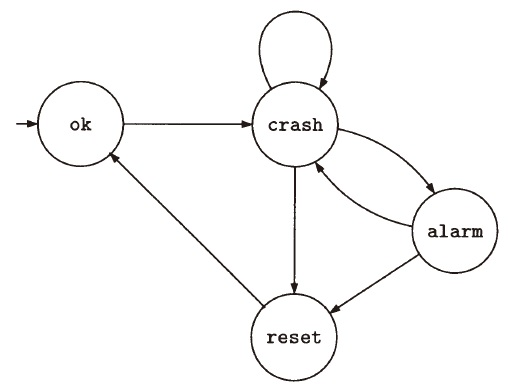
\includegraphics[width=3.0in, height=2.0in]{7_1.jpg}
            \caption{$\mathcal{A}$, a model of an alarm}
        \end{figure}
        And we need to guarantee three safety properties: $\textbf{AG}(\text{alarm}\Rightarrow\textbf{F}^{-1}\text{crash})$, $\textbf{AG}(\text{alarm}\Rightarrow(\neg\text{reset})\textbf{ S }\text{crash})$ and $\textbf{AG}(\text{alarm}\Rightarrow\textbf{X}^{-1}\text{crash})$. Since no current tool can handle past temporal logic, it needs another method to get rid of past formula $\phi^-$ and it is what history variables do. a history variable is a boolean variable and true if and only if $\phi^-$. Then it may update itself according to each transitions.
        
        For automaton $\mathcal{A}$, we can introduce history variable \textbf{h1} for $\textbf{AG}(\text{alarm}\Rightarrow\textbf{X}^{-1}\text{crash})$ and \textbf{h2} for $\textbf{AG}(\text{alarm}\Rightarrow(\neg\text{reset})\textbf{ S }\text{crash})$. Then update the value of \textbf{h1} and \textbf{h2}. For \textbf{h1}, it is initially false and updated to true each time when a transition from crash state to current state happens, otherwise, updated to false. And for \textbf{h2}, it is initially false and updated to true each time when a transition leads to crash state and to false each time when a transition leads to reset state, otherwise, leaving unchanged. In this way, we can transform the problem "does $\mathcal{A}\models\textbf{AG}(\text{alarm}\Rightarrow\textbf{X}^{-1}\text{crash})$" into $\mathcal{A}\models(\text{alarm}\Rightarrow\textbf{h1})$. And the resulting automaton $\mathcal{A}_{+\text{hist}}$ is as picture below shows.
        \begin{figure}[H]
            \centering
            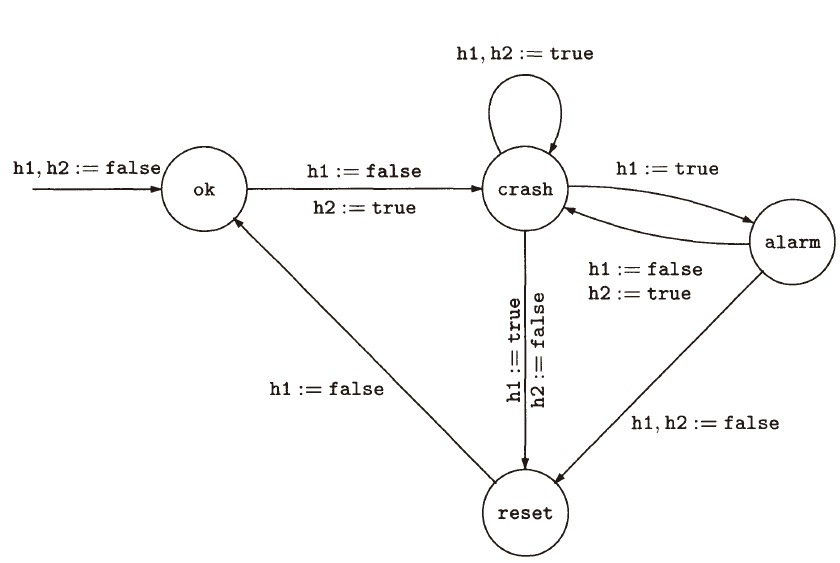
\includegraphics[width=4.0in, height=3.0in]{7_2.jpg}
            \caption{$\mathcal{A}_{+\text{hist}}$, the automaton $\mathcal{A}$ enriched with its history variables}
        \end{figure}
        
    \section{Summary}
        Chapter 6 and 7 introduces reachability properties and safety properties respectively. Reachability properties is simple and can be written in the form of $\textbf{EF}\phi$ where $\phi$ is a formula free of temporal combinators. We can compute reachability graph to verify reachability properties by forward chaining method or backward chaining method.
        
        As for safety properties, it can be divided into three categories: simple, without past and without explicit past. Introducing past relies on an assumption that once a safety property is violated, then it should notice and handle it immediately. And in this way we can only verify safety properties with information of past and without the information of future. Then we can use history variables to deal with past formula.

\end{document} 